\documentclass{beamer}
\usecolortheme{wolverine}

% math stuff
\usepackage{amsmath}
\usepackage{amsthm}
\usepackage{amssymb}
\usepackage{xcolor}

\usepackage{float}
\usepackage{subcaption}

% to insert images
\usepackage{graphicx}

% to correctly insert stressed characters
\usepackage[T1]{fontenc}
\usepackage[utf8]{inputenc}

\usepackage{multirow}

% Bibliography
% \usepackage[style=alphabetic]{biblatex}
% \usepackage[nottoc]{tocbibind}
% \usepackage{bibentry}
% \setcounter{biburllcpenalty}{9000}
% \usepackage{nameref}
% \addbibresource{slides.bib}

% to put links in table of contents
\usepackage{hyperref}
\hypersetup{colorlinks=false, %set true if you want colored links
	linktoc=all,     %set to all if you
}

\usepackage{mathtools}

% Add symbols
% \usepackage{textcomp}

% Add command for Real and Z sets
% \usepackage{dsfont}
% \newcommand{\Rset}{$\mathds{R}$}
% \newcommand{\Zset}{$\mathds{Z}$}

% Code highlighting
% \usepackage{minted}
% \usemintedstyle{perldoc}
% \setminted{
%     frame=single,
%     breaklines,
% }

% tikz figures
\usepackage{tikzit}
\input{style.tikzstyles}

% number rounding
\usepackage{siunitx}
\sisetup{round-mode=places,round-precision=5}

\definecolor{myyellow}{RGB}{225, 225, 0}

\title{Thesis notes}
\date{1st June}

% any code between @(...)@ is escaped back to LaTeX
% \lstset{escapeinside={@(}{)@}}

% algorithms
\usepackage[ruled,vlined]{algorithm2e}
% \newtheorem{theorem}{Theorem}

\begin{document}
\frame{\titlepage}

\begin{frame}[c]
	\frametitle{The Echo Chamber Problem}
	\textbf{Goal}: given an interaction graph $G$, find $U \subseteq V$ maximing

	\begin{equation}
		\xi (U) = \sum^{}_{C \in \hat{\mathcal{C}} } \sum^{}_{T[U] \in S_C (U)}
		(| T^{+} [U] | - | T^{-} [U] |)
	\end{equation}

	where $| T^{-} [U] |$ and $| T^{+} [U] |$ denotes the number of negative
	and positive edges induced in the subgraph, respectively.

	\bigskip

	The set of users maximing the expression is denoted as $\hat{U}$ and the
	corresponding score is $\xi(G)$
\end{frame}


\begin{frame}[c]
	\frametitle{The rounding algorithm}
	\begin{algorithm}[H]
		\SetAlgoLined
		$\hat{G} \leftarrow $ empty graph \;
		$\hat{V} \leftarrow $ vertices of $\hat{G}$ \;
		$S = 0$

		\ForEach{ $e_{ij}^{k} \in \tilde{E}$ }{
			$\hat{V} \leftarrow \hat{V} \bigcup \{ v_{i} \}$ \textbf{if} $v_i
				\not\in \hat{V}$ \;
			$\hat{V} \leftarrow \hat{V} \bigcup \{ v_{j} \}$ \textbf{if} $v_j
				\not\in \hat{V}$ \;

			$S \leftarrow {\xi}(\hat{V})  $ \;

			\ForEach{component $C$ in $\hat{G}$}{
				$S \leftarrow \xi(C)$ \;
			}
		}

		\Return highest S \;

		\caption{Rounding algorithm}
		\label{alg:algorithm_rounding}
	\end{algorithm}
\end{frame}

\begin{frame}[c]
	\frametitle{Example}
	\begin{figure}[htpb]
		\centering
		\tikzfig{tikz/original_original}
		\caption{The original graph}%
		\label{fig:name}
	\end{figure}
\end{frame}

\begin{frame}[c]
	\frametitle{Example}
	If many edges get the same value in the result of the relaxation, they are
	selected randomly

	\begin{figure}[htpb]
		\centering
		\tikzfig{tikz/original_positive}
		\caption{Only positive edges are reported, getting all value
			0.666}%
		\label{fig:name}
	\end{figure}

\end{frame}

\begin{frame}[c]
	\frametitle{Example}
	When the edge $e_{35}$ is added then the 2 communities cannot be
	reconstructed.

	\begin{figure}[htpb]
		\centering
		\tikzfig{tikz/original_positive}
		\caption{Only positive edges are reported, getting all value
			0.666}%
		\label{fig:name}
	\end{figure}
\end{frame}

\begin{frame}[c]
	\frametitle{Example}
	Let us suppose it is added in the first iteration. Then we have a situation
	as follows

	\begin{figure}[htpb]
		\centering
		\tikzfig{tikz/original_exec}
		% \caption{}%
		% \label{fig:name}
	\end{figure}

	We won't be able to find a whole community during the remaining iterations
	and the result may even be $U = \{ v_{3}, v_5\}$.
\end{frame}

\begin{frame}[c]
	\frametitle{Example}
	A "luckier" iteration would be the following

	\begin{figure}[htpb]
		\centering
		\tikzfig{tikz/original_exec_lucky}
		% \caption{}%
		% \label{fig:name}
	\end{figure}
\end{frame}

\begin{frame}[c]
	\frametitle{Effects on the results}
	Since the addition of positive cross-community edges degradates the result,
	we can generally improve the chances of finding better fits on the
	community

	\begin{itemize}
		\item Reducing the number of positive cross-community edges
		\item increasing the number of positive edges inside a community
		\item icreasing the number of threads in order to be less sensitive
		      to single edges
	\end{itemize}

\end{frame}

\begin{frame}[c]
	\frametitle{A model for the Echo Chamber Problem}
	Each node has a group assignment and there are probabilities of
	positive and negative edges $\omega _{rs}^{+}  $ and $\omega _{rs}^{+}  $,
	respectively.

	\begin{enumerate}
		\item Generate the \emph{follow} graph $G$ by using a SBM with parameters
		      $\{ \phi _{rs}  \}$.
		\item Each node can be active with probability $\beta_{a}  $
		\item Any active node activates his inactive neighbours in $G$ with
		      probability $\beta_n$
		      % \item Let $a_{i} $ be the number of \emph{active} neighbours of node
		      %     $i$ in $G$ and $m_{i} $ the number of neighbours of node $i$ in
		      %     $G$. Any node inactive from the previous step is activated with
		      %     probability $ \frac{a_i}{m_i} \beta _{n} $
		\item active nodes interact according to the categorical $(\omega _{rs}
			      ^{+}, \omega _{rs} ^{-}, 1 - \omega _{rs} ^{+} - \omega _{rs} ^{-})
		      $ otherwise (at least one of the 2 nodes is inactive) with
		      categorical $(\theta \omega _{rs} ^{+}, \theta \omega _{rs} ^{-}, 1
			      - \theta (\omega _{rs} ^{+} + \omega _{rs} ^{-}))$, $\theta \leq 1$
	\end{enumerate}

\end{frame}

\begin{frame}[c]
	\frametitle{A parametrized model (1)}
	Parameter choice:
	\begin{equation}
		\phi_{rs}  =
		\begin{cases}
			1 \; & \text{if } r = s  \\
			0 \; & \text{otherwise }
		\end{cases}
	\end{equation}
	Users follow other all and only users in the same community.

	\bigskip

	$\beta _{a} = 1$ , $\beta_{n} = 1 $: all users interact on each post.

	\begin{equation}
		\omega_{rs}^{+}   =
		\begin{cases}
			1 - x \;        & \text{if } r = s  \\
			\frac{x}{4}  \; & \text{otherwise }
		\end{cases}
		\omega_{rs}^{-}   =
		\begin{cases}
			x \;                & \text{if } r = s  \\
			\frac{1 - x}{4}  \; & \text{otherwise }
		\end{cases}
	\end{equation}

	This means that the probability of having an edge between two nodes in
	different communities is $1/4$.
\end{frame}

\begin{frame}[c]
	\frametitle{Clustering results}

	\begin{figure}[htpb]
		\centering
		\includegraphics[width=0.8\linewidth]{out/synthetic_appr/scores.png}
		\caption{Approximation algorithm scores}%
		\label{fig:out/synthetic_appr/scores}
	\end{figure}

	Results obtained with 8 nodes per community and 12 threads.

\end{frame}

\begin{frame}[c]
	\frametitle{More observations}
	The results clearly depends on factors like:
	\begin{itemize}
		\item the number of threads (the higher the number of threads the more
		      the algorithm is robust to noise),
		\item the number of nodes (the higher the number of nodes the more
		      the algorithm is robust to noise).
	\end{itemize}
\end{frame}
% \begin{frame}[c]
%     \frametitle{Clustering results}
%
%     \begin{figure}[htpb]
%         \centering
%         \includegraphics[width=0.8\linewidth]{out/synthetic_exact/scores.png}
%         \caption{Exact algorithm scores}%
%         \label{fig:out/synthetic_appr/scores}
%     \end{figure}
%
% \end{frame}
\end{document}
